\maketitle
\section{Signed binary numbers}

Signed numbers include both negative and positive numbers. There three common
signed number representations

\begin{enumerate}
\item Sign magnitude representation
\item One's complement
\item Two's complement
\end{enumerate}
  
\subsection{Sign-magnitude representation}
The Most significant (left most) \emph{bit} (binary digit) represents sign ($0 =
+$ and $1 = -$), the rest represent the magnitude. Example, a 5-bit number
$(11010)_2$ in signed magnitude representation has the value of $(-1010)_2 =
-10$. Note that $+10$ has to be represented by a leading $0$ at the most
significant bit (MSB) $+10 = (01010)_2$. Hence, the number of bits have to be specified.

\begin{prob}
  \begin{itemize}
\item Write down all possible 4-digit binary numbers and corresponding decimal
  values if they are in signed magnitude format? What is the minimum and maximum value?
  \item What is the minimum and maximum value of n-digit signed binary number in
    sign-magnitude format?
\end{itemize}
\end{prob}

%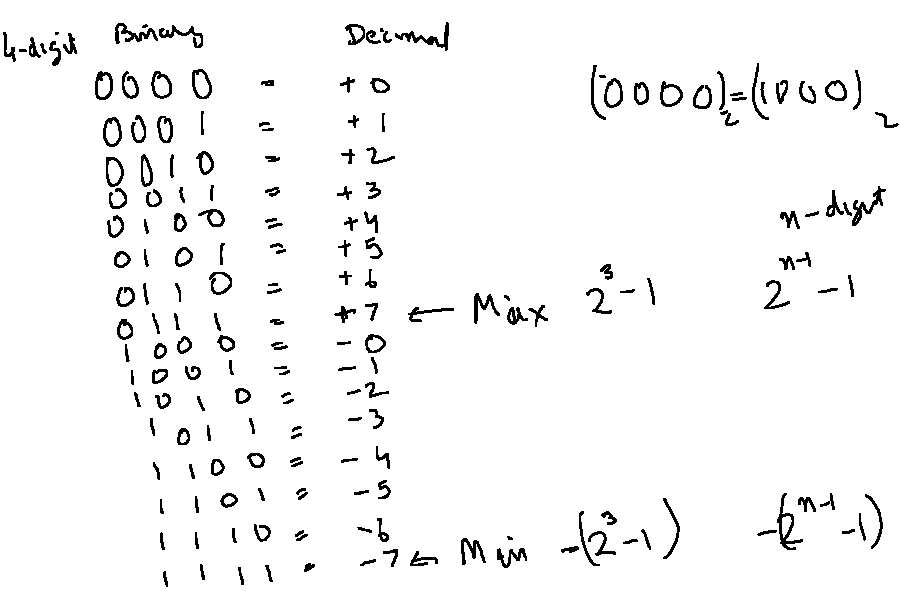
\includegraphics[width=12cm]{sign-magnitude-numbers.pdf}
\vspace{20em}

\subsection{One's complement negation}

You can convert a positive number (say +10) to negative number by applying a
negative sign in front of it (-(+10) = -10). It is more evident from taking
negative of a negative number (-(-10) = +10). In case of sign-magnitude
representation, the ``negative operator'' flips the sign bit. The next two
signed number representations (1's complement and 2's complement) are designed
around specific negative operator definitions.

\noindent Negate $13_{10} = 01101_2$ using 5-bit one's complement.
\vspace{10em}

\noindent Negate $-13_{10}$ using 5-bit one's complement.
\vspace{10em}

\subsection{One's complement binary numbers}

In one's complement representation, the negative operation is obtained by flipping
all the bits of the binary number. Example, a 5-bit one's
complement of $+10 = (01010)_2$ is $(10101)_2 = -10$. Note that flipping bits is
equivalent to subtracting the number from $(11111)_2$, hence the name. You can
also confirm that double negative operator yields back the same number.

\begin{prob}
  \begin{itemize}
  \item Write down all possible 4-digit binary numbers and corresponding decimal
    values if they are in sign magnitude format? What is the minimum and maximum value?
  \item What is the minimum and maximum value of n-digit signed binary number in
    one's complement?
  \end{itemize}
\end{prob}
\vspace{20em}

\begin{prob}
  Determine the decimal values of the following 1’s complement 6-digit binary numbers :
  \begin{enumerate}
  \item 01101110
  \item 10101101
  \end{enumerate}
\end{prob}
\vspace{20em}

\begin{prob}
  Convert the decimal numbers -17 and +23 into the 6-digit one's complement binary numbers and try adding them. What
  adjustments will you need to make to get the right result's (23-17=6) in binary representation.
\end{prob}
\vspace{20em}


\subsection{Two's complement negation}
In two's complement representation, the n-digit negative number is obtained by
subtracting the positive number from $2^{n}$. Example, two's
complement of 5-digit binary number $+10 = (01010)_2$ is $2^5 - 10 = 22 =
(11000)_2$. An easier algorithm to get two's complement goes via one's
complement. Note that $(11111)_2 = 2^5-1$. We can get two's complement by adding
1 to one's complement. To get two's complement:
\begin{enumerate}
\item Flip all the bits. (Same as taking one's complement).
\item Add 1 to the number.
\end{enumerate}

\noindent Negate $13_{10} = 01101_2$ using 5-bit two's complement.
\vspace{10em}

\noindent Negate $-13_{10}$ using 5-bit two's complement.
\vspace{10em}


How to convert one's complement number representation into sign-magnitude numbers?
\begin{enumerate}
\item Check if the number is positive or negative. Even for one's complement representation, or two's complement representation, if the MSB (Most-significant bit) is 1, then the number is negative, otherwise positive.
\item If positive: For positive numbers, two's complement, one's complement and sign magnitude are the same. No conversion between different representation is needed.
2.b If negative: For negative numbers. Flip the bits of 1's complement. Once you flip the 1's complement bits of a negative number, you get the corresponding positive number.
\item We still want to represent the original negative number. So we set the MSB of sign-magnitude representation to 1. Since the range (min and max) for both n-bit 1's complement and sign-magnitude are the same (between $-(2^{n-1}-1)$ and $2^{n-1}-1$), you can always represent 8-bit 1's complement numbers with needing to extend the 8-bit number to 9-bits.
\end{enumerate}

Example: Convert 8-bit one's complement 10101010 to 8-bit sign-magnitude
Let number n = 10101010
\begin{enumerate}
\item Is the number +ve or -ve: It is negative because it starts with 1.
\item The number is not positive.
\item Take the 1's complement of the negative number to get the positive part. i.e. Flip the bits:\\
-n = 01010101 or n = -(01010101)
\item
 We got the positive part of the number, but we want to represent the original negative number, so we set the MSB bit one. Hence, the equivalent sign-magnitude representation is:\\
n = 11010101
\end{enumerate}


\subsection{Two's complement representation}

% \begin{prob}
%   \begin{itemize}
%   \item Write down all possible 4-digit binary numbers and corresponding decimal
%     values if they are in two's complement format? What is the minimum and maximum value?
%   \item What is the minimum and maximum value of n-digit signed binary number in
%     two's complement?
%   \end{itemize}
% \end{prob}
\vspace{20em}

\begin{prob}
  Determine the decimal values of the following 2’s complement 6-digit numbers :
  \begin{enumerate}
  \item 01011110
  \item 10010111
  \end{enumerate}
\end{prob}
\vspace{10em}

\begin{prob}
  Convert the decimal numbers -17 and +23 into the 6-digit two's complement binary numbers and try adding them. What adjustments will you need to make to get the right result's (23-17=6) in binary representation.
\end{prob}
\vspace{20em}

\begin{prob}
  Convert the decimal numbers 73, 23, -17, and -163 into signed 8-bit numbers in the
  following representations:
  \begin{enumerate}
    \item Sign and magnitude
    \item 1’s complement
    \item 2’s complement
  \end{enumerate}
\end{prob}
\vspace{20em}


\subsection{Arithmetic overflow}
\begin{prob}
  Consider addition of 4-digit two's complement binary numbers
  \begin{enumerate}
  \item $1010_2 + 1101_2$
  \item $1011_2 + 1100_2$
  \end{enumerate}
  In which of the two case overflow happens? Can you come up with a rule to ``easily'' detect overflow?
\end{prob}
\vspace{20em}

\subsubsection{Rules for detecting arithmetic overflow:}

\begin{enumerate}
  \item Adding numbers of different signs never produces an overflow.
  \item Adding numbers of the same sign may produce an overflow
    \begin{enumerate}
        \item Wrong approach: Adding two negative 2's complement numbers always produces an additional carry-over 1, but that in itself isn't an overflow. An example, the range of 4-bit 2's complement numbers is between -8 to +7. Adding -3 to -4 in 2's complement is 1101 + 1100 produces an additional carry over 1. You can ignore the additional carry-over 1 to get the correct answer 1001 = -7 which is within range -8 to 7.
        \item Approach 1: The easiest way for now to detect overflow is if adding two -ve numbers results in a +ve number, or adding +ve numbers results in a -ve number.
        \item Approach 2: You can also do a range test in decimal based range test. The range of n-bit 2's complement numbers is between $-2^{n-1}$ and $2^{n-1}-1$. For 5-bit 2's complement numbers, it is between -16 and 15. For 6-bit 2's complement numbers, it is between -32 and 31.
        \item Approach 3: You can also check the carry-overs of the most significant two bits. If they match, i.e. 0 and 0, or 1 and 1, then there is no overflow. If they do not match, i.e. 0 and 1 or 1 and 0, then there is an overflow.
     \end{enumerate}
\end{enumerate}



\section{Binary coded decimal}
In Binary coded decimal (BCD), each decimal digit is represented by 4 bits. For
example, $1047 = (0001\_0000\_0100\_0111)_{\text{BCD}}$. It is useful in
input-output applications where the number has to be either displayed as decimal
or received as decimal.

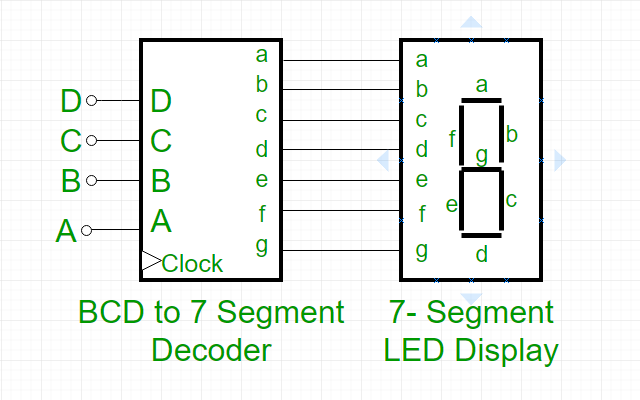
\includegraphics[width=0.5\linewidth]{bcdto7seg.png}

\begin{prob}
  Convert 11, 23, 35, 57 and 103897 to BCD?
\end{prob}
\vspace{10em}

\section{Gray code}
A sequence of binary numbers where only one bit changes when the number
increases by 1. It is helpful in applications like wheel encoders


\includegraphics[width=0.5\linewidth]{gray-code.pdf}

\begin{prob}
  Write all possible 3-bit binary numbers in gray-code
\end{prob}
\vspace{10em}
